\documentclass[aspectratio=1610]{beamer}

\usepackage{graphicx}
\usepackage[english]{babel}
\usepackage[T1]{fontenc}
\usepackage{csquotes, xcolor, xspace, changepage, setspace, listings}
\usepackage{libertinus}
\usepackage{roboto, anyfontsize}
\usepackage{fontawesome5}
\usepackage[scale = 0.75]{plex-mono}
\usepackage{tikz, subcaption}

\usetikzlibrary{fit, shapes.geometric, shapes.symbols, positioning, shapes.misc, calc, arrows.meta, patterns, backgrounds, decorations, decorations.markings, decorations.pathreplacing, shadows, hobby}

\usepackage[backend=bibtex,style=authoryear]{biblatex}
\addbibresource{biblio.bib}

\title{Real-Time Analysis of Public GitHub Activity}
\author{Roland Bernard}
\date{Febuary 2026}

\definecolor{unibzblue}{HTML}{0086ec}
\definecolor{unibzblue2}{HTML}{f0f8ff}

\setbeamercolor{outerbox}{fg=black,bg=unibzblue2}
\setbeamercolor{innerbox}{fg=white,bg=unibzblue}

\setbeamertemplate{title page}{
  \scriptsize 
  \begin{tabular}{ll}
    \vspace*{40mm} \\
    \multicolumn{2}{l}{\raggedright Final Presentation -- Real-Time Big Data Processing 2024/2025} \\
    \\
    \multicolumn{2}{p{\linewidth}}{\raggedright \fontsize{18}{20}\selectfont \bf \inserttitle} \\
    \\
    \\
    & \insertauthor \\
    \\
    & \insertdate \\
  \end{tabular}
}

\setbeamertemplate{frametitle}{
  \vspace*{6mm}
  \Large \bf \color{black} \insertframetitle
}

\setbeamertemplate{itemize items}{\scriptsize\raisebox{0.6mm}{\color{unibzblue} $\blacktriangleright$}}

\beamertemplatenavigationsymbolsempty
\setbeamertemplate{footline}{
  \begin{beamercolorbox}[wd=\paperwidth,right]{section in head/foot}
    \usebeamerfont{date in head/foot}\hspace*{2em}
    \insertframenumber{}\hspace*{2mm} 
    \vspace*{2mm}
  \end{beamercolorbox}
}

\newcommand{\litem}{{\scriptsize\raisebox{0.6mm}{\color{unibzblue} $\blacktriangleright$}}}
\newcommand{\sitem}{{\scriptsize\raisebox{0.2mm}{\color{unibzblue} $\rightarrow$}}\enspace}
\newcommand{\icon}[1]{\textcolor{unibzblue}{\faIcon[solid]{#1}}}

\newlength{\offsetpage}
\newenvironment{narrowpage}[1][3mm]{
  \setlength{\offsetpage}{#1}
  \begin{adjustwidth}{\offsetpage}{\offsetpage}
}{
  \end{adjustwidth}
}
\newenvironment{widepage}[1][10mm]{
  \setlength{\offsetpage}{#1}
  \begin{adjustwidth}{-\offsetpage}{-\offsetpage}
}{
  \end{adjustwidth}
}

\newenvironment{items}{
  \begin{narrowpage}
}{
  \end{narrowpage}
}
\newenvironment{oitem}[2][3mm]{
  \vspace*{2mm}
  \begin{beamercolorbox}[rounded=false,colsep=#1]{outerbox}
    \parbox[t]{2mm}{\centering#2}\parbox[t]{2mm}{\ }%
    \begin{minipage}[t]{\linewidth}
}{
    \end{minipage}
  \end{beamercolorbox}
  \vfill
}

\definecolor{unibzblue}{HTML}{0086ec}
\definecolor{unibzblue2}{HTML}{f0f8ff}

\pgfdeclarelayer{background}
\pgfdeclarelayer{foreground}
\pgfsetlayers{background,main,foreground}

\tikzset{
  flow/.style={-{Triangle[length=6, width=6]}, draw=red!70!black, very thick, shorten >= -3},
  biflow/.style={flow, {Triangle[length=6, width=6]}-{Triangle[length=6, width=6]}},
  link/.style={->, draw},
  ptr/.style={->, dashed},
  leafl/.style={-, thick},
  external/.style={inner sep=10, draw=black, fill=brown!20},
  internal/.style={inner sep=10, draw=black, fill=unibzblue!20},
  build/.style={inner sep=10, draw=black, fill=unibzblue!40},
  mixed/.style={inner sep=8.7, draw=black, path picture={
    \fill[brown!20] (path picture bounding box.south west)
      rectangle ($(path picture bounding box.north west)!.675!(path picture bounding box.north east)$);
    \fill[unibzblue!40] ($(path picture bounding box.north west)!.675!(path picture bounding box.north east)$)
      rectangle (path picture bounding box.south east);
  }},
  >=Latex, node distance=1, every node/.style={inner sep=0}
}


\begin{document}

\begin{frame}[plain]
  \input{tikzfigures/title.tex}
  \titlepage
\end{frame}

\begin{frame}
\frametitle{Application Domain}
  \begin{items}
    \begin{oitem}{\litem}
      Motivation and Context: \\
      \sitem {\footnotesize GitHub hosts millions of developers and repositories.} \\
      \sitem {\footnotesize Generates large volumes of public events.} \\
      \sitem {\footnotesize Most existing tools focus mainly on historical analysis.}
    \end{oitem}
    \begin{oitem}{\litem}
      Project Objectives: \\
      \sitem {\footnotesize Collect GitHub events continuously.} \\
      \sitem {\footnotesize Process data in real time.} \\
      \sitem {\footnotesize Provide interactive dashboard.} \\
      \sitem {\footnotesize Ensure low latency and reliability.}
    \end{oitem}
    \begin{center}
      \begin{tikzpicture}[
          node distance=10mm,>=Latex,
          base_node/.style={minimum height=5mm,align=center,text width=3cm},
          icon_node/.style={minimum size=7mm,align=center}
      ]
          \node (satellite) [icon_node] {\fontsize{40pt}{40pt}\selectfont\faGithub};
          \node [base_node, right=of satellite, inner sep=-5mm, yshift=10, xshift=10, text=yellow] {\fontsize{20pt}{20pt}\selectfont\faStar};
          \node (image_data) [base_node, right=of satellite, inner sep=-5mm, text=red] {\fontsize{20pt}{20pt}\selectfont\faCodeBranch};
          \node [base_node, right=of satellite, inner sep=-5mm, yshift=-10, xshift=-10] {\fontsize{20pt}{20pt}\selectfont\faCode};
          \node [below=6.25mm of image_data, font=\scriptsize] {Raw Events};
          \node (machine_learning) [icon_node, right=of image_data] {\fontsize{40pt}{40pt}\selectfont\faServer};
          \node [below=1mm of machine_learning, font=\scriptsize] {Real-time Processing};
          \node [base_node, right=of machine_learning, inner sep=-5mm, yshift=4, xshift=4] {\includegraphics[width=20mm]{figures/repo.png}};
          \node [base_node, right=of machine_learning, inner sep=-5mm, yshift=2, xshift=2, rounded corners] {\includegraphics[width=20mm]{figures/events.png}};
          \node (pred) [base_node, right=of machine_learning, inner sep=-5mm] {\includegraphics[width=20mm]{figures/insights.png}};
          \node [below=6.25mm of pred, font=\scriptsize] {Interactive UI};
          \draw[->, thick] (satellite) -- (image_data);
          \draw[->, thick] (image_data) -- (machine_learning);
          \draw[->, thick] (machine_learning) -- (pred);
      \end{tikzpicture}
    \end{center}
  \end{items}
\end{frame}

\begin{frame}[fragile]
\frametitle{Description of the Data Sources}
  \begin{columns}
    \column{0.67\linewidth}
    \begin{items}
      \begin{oitem}{\litem}
        GitHub Events API: \\
        \sitem {\footnotesize Endpoint: \url{https://api.github.com/events.}} \\
        \sitem {\footnotesize Up to 300 most recent public events in JSON format.} \\
        \sitem {\footnotesize Rate limited, i.e., access token required.}
      \end{oitem}
      \begin{oitem}{\litem}
        Key Properties: \\
        \sitem {\footnotesize Variety: many event types, e.g., push, issues, stars, etc.} \\
        \sitem {\footnotesize Velocity: up to 120 events/sec, millions of events per day.} \\
        \sitem {\footnotesize Veracity: out-of-order and delayed events.} \\
        \sitem {\footnotesize Latency: API around 5 minutes behind real time.}
      \end{oitem}
    \end{items}
    \column{0.33\linewidth}
    \vspace{-13mm}
    \begin{figure}
      \scriptsize
\begin{verbatim}
{
  "id": "8251545586",
  "type": "PushEvent",
  "actor": {
    "id": 121951544,
    "login": "movieflixgr",
    "display_login": "movieflixgr",
    "gravatar_id": "",
    "url": "https://api.github.com/users/[..]",
    "avatar_url": "https://avatars.github[..]"
  },
  "repo": {
    "id": 1126450259,
    "name": "movieflixgr/Subtitles",
    "url": "https://api.github.com/repos/[..]"
  },
  "payload": {
    "repository_id": 1126450259,
    "push_id": 30546526697,
    "ref": "refs/heads/main",
    "head": "d5e986993aa47729cb18a82ac9d1[..]",
    "before": "6bf91f2d0600084cc7218c1934[..]"
  },
  "public": true,
  "created_at": "2026-02-08T20:09:50Z"
}
\end{verbatim}
    \end{figure}
  \end{columns}
\end{frame}

\begin{frame}
\frametitle{System Architecture}
  \begin{items}
    \begin{oitem}{\litem}
      Technology Stack: \\
      \sitem {\footnotesize Backend: Java + Maven; RxJava; Apache Kafka; Apache Flink; PostgreSQL + TimescaleDB} \\
      \sitem {\footnotesize Frontend: Single Page Application with React + TypeScript; Vite; Recharts; RxJS} \\
      \sitem {\footnotesize Deployment: Docker and Docker Compose}
    \end{oitem}
    \begin{widepage}
      \begin{center}
        \begin{figure*}[ht]
  \centering
  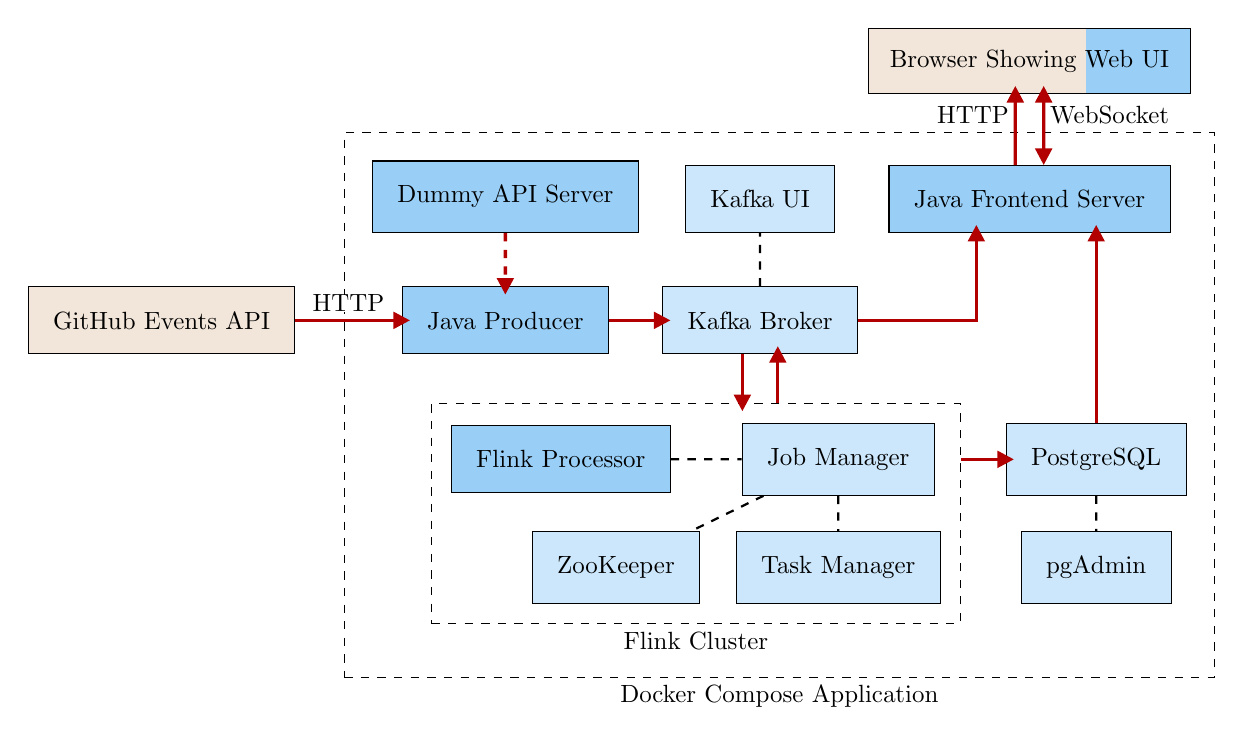
\begin{tikzpicture}[scale=0.9, transform shape]
    \node[external] (github) {GitHub Events API};
    \node[build, right=1.5 of github] (producer) {Java Producer};
    \draw[flow] (github) -> (producer) node [midway, fill=white, above=0.1] {HTTP};
    \node[internal, right=0.75 of producer] (kafka) {Kafka Broker};
    \draw[flow] (producer) -> (kafka);
    \node[internal, above=0.75 of kafka] (kafkaui) {Kafka UI};
    \draw[dashed, thick] (kafka) -> (kafkaui);
    \node[build, below=of kafka, xshift=-80] (processor) {Flink Processor};
    \node[internal, right=of processor] (jobmanager) {Job Manager};
    \draw[dashed, thick] (processor) -> (jobmanager);
    \node[internal, below=0.5 of jobmanager] (taskmanager) {Task Manager};
    \draw[dashed, thick] (jobmanager) -> (taskmanager);
    \node[internal, left=0.5 of taskmanager] (zookeeper) {ZooKeeper};
    \draw[dashed, thick] (jobmanager) -> (zookeeper);
    \begin{scope}[on background layer]
      \node[draw, dashed, fit=(processor)(jobmanager)(taskmanager), inner sep=7] (flink) {};
      \node[below=0.1 of flink] (flinklabel) {Flink Cluster};
    \end{scope}
    \draw[flow] ($(kafka.south)-(0.25,0)$) -> ($(kafka |- flink.north)-(0.25,0)$);
    \draw[flow] ($(kafka |- flink.north)+(0.25,0)$) -> ($(kafka.south)+(0.25,0)$);
    \node[build, above=0.75 of producer] (dummy) {Dummy API Server};
    \draw[flow, dashed] (dummy) -> (producer);
    \node[build, right=0.75 of kafkaui] (frontend) {Java Frontend Server};
    \draw[flow] (kafka) -| ($(frontend.south)-(0.75,0)$);
    \node[internal, right=of jobmanager] (postgres) {PostgreSQL};
    \node[internal, below=0.5 of postgres] (pgadmin) {pgAdmin};
    \draw[dashed, thick] (postgres) -- (pgadmin);
    \draw[flow] ($(postgres -| flink.east)$) -> ($(postgres.west)$);
    \draw[flow] ($(postgres.north)$) -> ($(postgres |- frontend.south)$);
    \node[mixed, above=of frontend] (browser) {Browser Showing Web UI};
    \draw[flow] ($(frontend.north)-(0.2,0)$) -> ($(browser.south)-(0.2,0)$) node [midway, fill=white, above left=0.1] {HTTP};
    \draw[biflow] ($(frontend.north)+(0.2,0)$) -> ($(browser.south)+(0.2,0)$) node [midway, fill=white, above right=0.1] {WebSocket};
    \begin{scope}[on background layer]
      \node[draw, dashed, fit=(flink)(flinklabel)(producer)(kafkaui)(frontend)(dummy)(postgres), inner sep=10] (docker) {};
      \node[below=0.1 of docker] (dockerlabel) {Docker Compose Application};
    \end{scope}
  \end{tikzpicture}
  \caption{Implemented application architecture. Blue indicates parts of the architecture controlled by the project, while the brown indicates external components. Darker blue represents components implemented as part of the project, while light blue components represent the use of existing software that has merely been configured.}
  \label{fig:arch}
\end{figure*}

      \end{center}
    \end{widepage}
  \end{items}
\end{frame}

\begin{frame}
\frametitle{System Architecture -- Data Ingestion}
  \begin{items}
    \begin{oitem}{\litem}
      Kafka Producer: \\
      \sitem {\footnotesize Polls GitHub API periodically, respecting rate limits.} \\
      \sitem {\footnotesize Retrieves overlapping windows, then deduplicates events.} \\
      \sitem {\footnotesize Publishes deduplicated events to Kafka topic.}
    \end{oitem}
    \begin{oitem}{\litem}
      Testing Mode: \\
      \sitem {\footnotesize Dummy API server to simulate real GitHub API with configurable throughput.}
    \end{oitem}
    \begin{center}
      \input{tikzfigures/ingest.tex}
    \end{center}
  \end{items}
\end{frame}

\begin{frame}
\frametitle{System Architecture -- Messaging}
  \begin{items}
    \begin{oitem}{\litem}
      Apache Kafka: \\
      \sitem {\footnotesize Decouples the ingestion from the processing.} \\
      \sitem {\footnotesize Decouples the processing from the frontend.} \\
      \sitem {\footnotesize Kafka message retention enables restarting Flink job without losing events.}
    \end{oitem}
    \begin{center}
      \input{tikzfigures/kafka.tex}
    \end{center}
  \end{items}
\end{frame}

\begin{frame}
\frametitle{System Architecture -- Stream Processing}
  \begin{items}
    \begin{oitem}{\litem}
      Core Processing Tasks: \\
      \sitem {\footnotesize Retrieve raw events from Kafka an parse JSON.} \\
      \sitem {\footnotesize Event-time processing using Watermarks with 10s maximum out-of-orderness.} \\
      \sitem {\footnotesize Writes results to PostgreSQL and Kafka.}
    \end{oitem}
    \begin{oitem}{\litem}
      Windowed Aggregations: \\
      \sitem {\footnotesize Tumbling windows with 10s and 5min window sizes.} \\
      \sitem {\footnotesize Custom sliding windows with 5min, 1h, 6h, and 24h length, updated every second.}
    \end{oitem}
    \begin{center}
      \input{tikzfigures/processing.tex}
    \end{center}
  \end{items}
\end{frame}

\begin{frame}
\frametitle{System Architecture -- Stream Processing}
  \begin{items}
    \begin{oitem}{\litem}
      Leaderboards: \\
      \sitem {\footnotesize User and repository activity ranking.} \\
      \sitem {\footnotesize Based on latest values from sliding window aggregations.} \\
      \sitem {\footnotesize Optimization: Emits only changed rows and frontend reconstructs ranking.}
    \end{oitem}
    \begin{oitem}{\litem}
      Trending Score: \\
      \sitem {\footnotesize Weighted sum of recent stars: \quad $t_\mathrm{score} = 10 s_{5\mathrm{m}} + 5 s_{5\mathrm{h}} + 2 s_{6\mathrm{h}} + s_{24\mathrm{h}}$.}
    \end{oitem}
    \begin{center}
      \input{tikzfigures/processing.tex}
    \end{center}
  \end{items}
\end{frame}

\begin{frame}
\frametitle{System Architecture -- Storage}
  \begin{items}
    \begin{oitem}{\litem}
      PostgreSQL + TimescaleDB: \\
      \sitem {\footnotesize Persistent storage for results of Flink processor.} \\
      \sitem {\footnotesize Handles queries for initial snapshot and historical data.} \\
      \sitem {\footnotesize Makes use of TimescaleDB hypertables and retention policy.} \\
      \sitem {\footnotesize Database commit before Kafka publish to ensure consistency.}
    \end{oitem}
    \begin{center}
      \begin{figure}
  \centering
  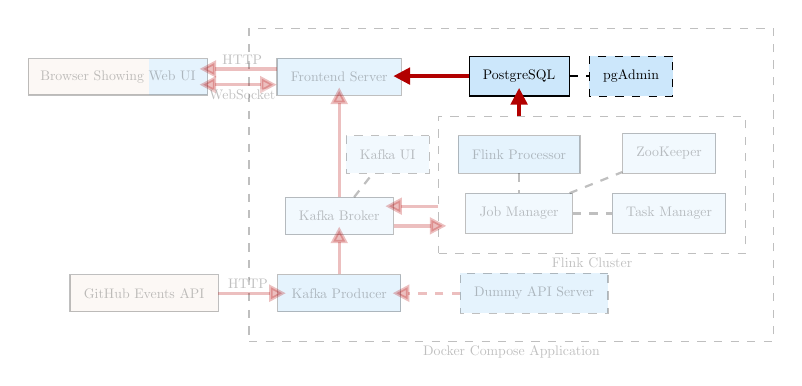
\begin{tikzpicture}[scale=0.5, transform shape, every path/.style={opacity=0.25}]
    \node[external] (github) {GitHub Events API};
    \node[build, right=1.5 of github] (producer) {Kafka Producer};
    \draw[flow] (github) -> (producer) node [midway, fill=white, above=0.1] {HTTP};
    \node[internal, above=of producer] (kafka) {Kafka Broker};
    \draw[flow] (producer) -> (kafka);
    \node[internal, dashed, above=0.6 of kafka, xshift=35] (kafkaui) {Kafka UI};
    \draw[dashed, thick] (kafka) -> (kafkaui);
    \node[build, above=0.6 of kafka, xshift=130] (processor) {Flink Processor};
    \node[internal, below=0.5 of processor] (jobmanager) {Job Manager};
    \draw[dashed, thick] (processor) -> (jobmanager);
    \node[internal, right=of jobmanager] (taskmanager) {Task Manager};
    \draw[dashed, thick] (jobmanager) -> (taskmanager);
    \node[internal, above=0.5 of taskmanager] (zookeeper) {ZooKeeper};
    \draw[dashed, thick] (jobmanager) -> (zookeeper);
    \begin{scope}[on background layer]
      \node[draw, dashed, fit=(processor)(jobmanager)(taskmanager), inner sep=7] (flink) {};
      \node[below=0.1 of flink] (flinklabel) {Flink Cluster};
    \end{scope}
    \draw[flow] ($(kafka.east)-(0,0.25)$) -> ($(kafka -| flink.west)-(0,0.25)$);
    \draw[flow] ($(kafka -| flink.west)+(0,0.25)$) -> ($(kafka.east)+(0,0.25)$);
    \node[build, dashed, right=1.5 of producer] (dummy) {Dummy API Server};
    \draw[flow, dashed] (dummy) -> (producer);
    \node[build, above=2.575 of kafka] (frontend) {Frontend Server};
    \draw[flow] (kafka) -> ($(kafka |- frontend.south)$);
    \node[internal, above=of processor, opacity=1] (postgres) {PostgreSQL};
    \node[internal, dashed, right=0.5 of postgres, opacity=1] (pgadmin) {pgAdmin};
    \draw[dashed, thick, opacity=1] (postgres) -- (pgadmin);
    \draw[flow, opacity=1] ($(postgres |- flink.north)$) -> ($(postgres.south)$);
    \draw[flow, opacity=1] ($(postgres.west)$) -> ($(postgres -| frontend.east)$);
    \node[mixed, left=1.75 of frontend] (browser) {Browser Showing Web UI};
    \draw[flow] ($(frontend.west)+(0,0.2)$) -> ($(browser.east)+(0,0.2)$) node [midway, fill=white, above=0.1] {HTTP};
    \draw[biflow] ($(frontend.west)-(0,0.2)$) -> ($(browser.east)-(0,0.2)$) node [midway, fill=white, below=0.1] {WebSocket};
    \begin{scope}[on background layer]
      \node[draw, dashed, fit=(flink)(flinklabel)(producer)(kafkaui)(frontend)(dummy)(postgres), inner sep=10] (docker) {};
      \node[below=0.1 of docker] (dockerlabel) {Docker Compose Application};
    \end{scope}
  \end{tikzpicture}
\end{figure}

    \end{center}
  \end{items}
\end{frame}

\begin{frame}
\frametitle{System Architecture -- Data Serving}
  \begin{items}
    \begin{oitem}{\litem}
      Frontend Server: \\
      \sitem {\footnotesize HTTP server for serving static files of the client web application.} \\
      \sitem {\footnotesize WebSocket server to serve API.} \\
      \sitem {\footnotesize Combines database queries for snapshots and Kafka streams for real-time updates.} \\
      \sitem {\footnotesize Manages client subscriptions to route events received from Kafka.}
    \end{oitem}
    \begin{center}
      \begin{figure}
  \centering
  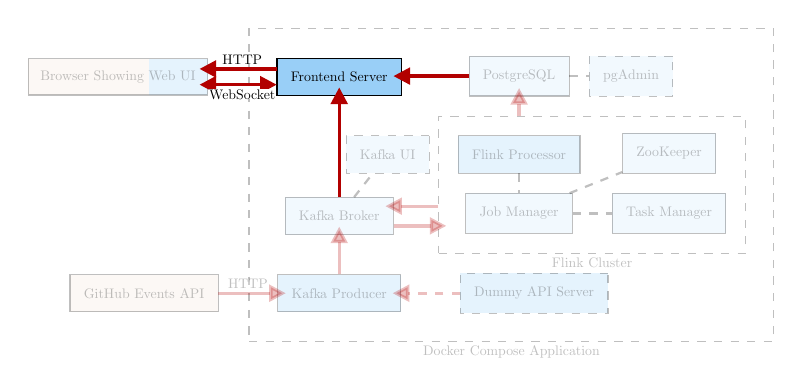
\begin{tikzpicture}[scale=0.5, transform shape, every path/.style={opacity=0.25}]
    \node[external] (github) {GitHub Events API};
    \node[build, right=1.5 of github] (producer) {Kafka Producer};
    \draw[flow] (github) -> (producer) node [midway, fill=white, above=0.1] {HTTP};
    \node[internal, above=of producer] (kafka) {Kafka Broker};
    \draw[flow] (producer) -> (kafka);
    \node[internal, dashed, above=0.6 of kafka, xshift=35] (kafkaui) {Kafka UI};
    \draw[dashed, thick] (kafka) -> (kafkaui);
    \node[build, above=0.6 of kafka, xshift=130] (processor) {Flink Processor};
    \node[internal, below=0.5 of processor] (jobmanager) {Job Manager};
    \draw[dashed, thick] (processor) -> (jobmanager);
    \node[internal, right=of jobmanager] (taskmanager) {Task Manager};
    \draw[dashed, thick] (jobmanager) -> (taskmanager);
    \node[internal, above=0.5 of taskmanager] (zookeeper) {ZooKeeper};
    \draw[dashed, thick] (jobmanager) -> (zookeeper);
    \begin{scope}[on background layer]
      \node[draw, dashed, fit=(processor)(jobmanager)(taskmanager), inner sep=7] (flink) {};
      \node[below=0.1 of flink] (flinklabel) {Flink Cluster};
    \end{scope}
    \draw[flow] ($(kafka.east)-(0,0.25)$) -> ($(kafka -| flink.west)-(0,0.25)$);
    \draw[flow] ($(kafka -| flink.west)+(0,0.25)$) -> ($(kafka.east)+(0,0.25)$);
    \node[build, dashed, right=1.5 of producer] (dummy) {Dummy API Server};
    \draw[flow, dashed] (dummy) -> (producer);
    \node[build, above=2.575 of kafka, opacity=1] (frontend) {Frontend Server};
    \draw[flow, opacity=1] (kafka) -> ($(kafka |- frontend.south)$);
    \node[internal, above=of processor] (postgres) {PostgreSQL};
    \node[internal, dashed, right=0.5 of postgres] (pgadmin) {pgAdmin};
    \draw[dashed, thick] (postgres) -- (pgadmin);
    \draw[flow] ($(postgres |- flink.north)$) -> ($(postgres.south)$);
    \draw[flow, opacity=1] ($(postgres.west)$) -> ($(postgres -| frontend.east)$);
    \node[mixed, left=1.75 of frontend] (browser) {Browser Showing Web UI};
    \draw[flow, opacity=1] ($(frontend.west)+(0,0.2)$) -> ($(browser.east)+(0,0.2)$) node [midway, fill=white, above=0.1] {HTTP};
    \draw[biflow, opacity=1] ($(frontend.west)-(0,0.2)$) -> ($(browser.east)-(0,0.2)$) node [midway, fill=white, below=0.1] {WebSocket};
    \begin{scope}[on background layer]
      \node[draw, dashed, fit=(flink)(flinklabel)(producer)(kafkaui)(frontend)(dummy)(postgres), inner sep=10] (docker) {};
      \node[below=0.1 of docker] (dockerlabel) {Docker Compose Application};
    \end{scope}
  \end{tikzpicture}
\end{figure}

    \end{center}
  \end{items}
\end{frame}

\begin{frame}
\frametitle{System Architecture -- Frontend}
  \begin{items}
    \begin{oitem}{\litem}
      Web Application: \\
      \sitem {\footnotesize A filterable live event stream.} \\
      \sitem {\footnotesize WebSocket server to serve API.} \\
      \sitem {\footnotesize Real-time counters for event volumes.} \\
      \sitem {\footnotesize User and repository leaderboards.}
    \end{oitem}
    \begin{center}
      \input{tikzfigures/browser.tex}
    \end{center}
  \end{items}
\end{frame}

\begin{frame}
\frametitle{Functionalities and Demo}
  \begin{items}
    \begin{oitem}{\litem}
      Live Demo: {\small \url{https://rtgh.rolandb.com}}
    \end{oitem}
  \end{items}
  \begin{widepage}
    \begin{center}
      \begin{tikzpicture}[node distance=5mm,>=Latex]
        \node (query) {
          \includegraphics[width=.33\textwidth]{figures/dashboard.png}};
        \node (ir_system) [right=of query, yshift=-30] {
          \includegraphics[width=.33\textwidth]{figures/events.png}};
        \node (results) [right=of ir_system, yshift=-30] {
          \includegraphics[width=.33\textwidth]{figures/repo.png}};
        \draw[flow] (query) -- (ir_system);
        \draw[flow] (ir_system) -- (results);
      \end{tikzpicture}
    \end{center}
  \end{widepage}
\end{frame}

\begin{frame}
\frametitle{Conclusion}
  \begin{items}
    \begin{oitem}{\litem}
      Successes: \\
      \sitem {\footnotesize Robust architecture able to handle 70-120 events per second.} \\
      \sitem {\footnotesize Docker and Docker Compose simplifies deployment.} \\
      \sitem {\footnotesize Responsive UI with leaderboards and charts updated in real-time.}
    \end{oitem}
    \begin{oitem}{\litem}
      Challenges: \\
      \sitem {\footnotesize Real-time rankings and long sliding window efficiency.} \\
      \sitem {\footnotesize API changes made by GitHub reduced information.} \\
      \sitem {\footnotesize Debugging Flink operator logic and state management.}
    \end{oitem}
    \begin{oitem}{\litem}
      Future Improvements: \\
      \sitem {\footnotesize More advanced models to detect trending repositories.} \\
      \sitem {\footnotesize Social media integration to see where repositories or users are mentioned.} \\
      \sitem {\footnotesize Sentiment analysis on the text content of certain event types.}
    \end{oitem}
  \end{items}
\end{frame}

{
\setbeamercolor{background canvas}{bg=black}
\begin{frame}[plain]{}
\end{frame}
}

\end{document}
